%\documentclass[a4paper,titlepage,12pt,DIV10,BCOR0.5cm,headinclude]{scrbook}
\documentclass[a4paper,titlepage,12pt,DIV10,BCOR0.5cm,headinclude]{article}
\DeclareFixedFont{\MyCode}{T1}{pcr}{m}{n}{10pt}
\usepackage[latin1]{inputenc}
\usepackage[T1]{fontenc}
\usepackage{eurosym}
\usepackage[pdftex]{graphicx}
\usepackage{ae}
%\usepackage{a4}	for scrbook
\usepackage{lscape}
% \usepackage{url}
\usepackage{listings}
\lstset{numbers=none, numberstyle=\tiny, numbersep=5pt}
\lstset{language=xml}

\pagestyle{plain}
\pagenumbering{arabic}


\begin{document}
\parindent 0pt

\tableofcontents
\newpage
%**************************************************************************************
\section{Introduction}
%**************************************************************************************
\textit{Information processing systems have grown up around the globe at "Web speed", only slightly slower than "warp speed" in science fiction.} \cite{Luckham05}
\\\\
The backbone of IT systems used in todays life are based on distributed systems that are wired together by the global spanning Internet. The Internet has become the foundation of the twenty-first-centuries daily business and increased the volume of information passed beween enterprises and rose the demand for shorter decision-making cycles significantly. Based on this distributed computing architecture banks, insureance companies, governments, hospitals, military, airports and many more use these technologies as a result of growing needs to reduce costs, increase competitiveness and increase the time to market. Almost no enterprise can go around those technologies in daily life without a loss of competitiveness even if it is only the basic communication facility like the email service deployed.
\\\\
\textit{A distribute system is a collection of independent computers that appears to its users as a single coherent system.} [Tanenbaum1]
\\\\
The world has become a global market and the Internet is the highway connecting each other on the globe. On a virtual global trade market a bunch of enterprises are connected together so they can share resources or automate trading process to fullfill the needs for flexibility on a global market. E-Commerce processes became more and more complex and highly asynchronous. Enterprise systems supporting a wide range of enterprise collaborations including managment support tasks like supply chain managment (SCM), business intelligence (BI) in general or enterprise resource planning systems (ERP). The typical application in this infrastructure is to automate the workflows of commercial enterprises like transaction processing in the financial sector or the general support of electronic collaborations. As business process have grown out traditional synchronous workflow to support electronic collaborations, especially in B2B markets, more sophisitcated techniques have been developed to support them. E-business processes became complex, highly parallel and asynchronouse with far less human involment \cite{LuckhamManensPark}. 
\\\\
\textit{Today thousands of business-level events per second are being communicated across the IT layers of some enterprises. These numbers will increase with activity in the global eMarketplace.} [Luckham06]
\\\\
For example an auto manufacturer can automatically place orders around the globe for specific parts and receive delivery offers so that the production can be done in a "just in time" manner without the time consuming and error prone work of humans while he is reducing the inventory costs. Furthermore this way of doing business is fast and unchallengeable cheap. These collaboration may manifest in either a horizontal way or vertical way. The horizontal collaboration is restricted to a specific industry where business is centered around hubs. The vertical is opened to different clients that can purchase goods from a supplier. More typical applications are the well known Supply Chain Managment or Enterprise Resource Planning. Almost every deparment can benefit from these systems like marketing with CRM applications, the manangment by business intelligence informations and ERP systems, the sales and buying department using supply chain managment systems and so on. As you can see not every application must go out of the enterprises bounds.
\\\\
The main benefit of this so called "enterprise systems" are:
\begin{itemize}
	\item reduced costs
	\item lower inventory levels
	\item faster time to market
	\item increase profitability
	\item increate competitiveness
\end{itemize}
The main drawback of such systems is that they are "event driven" systems where billions of events on different granularity levels fly across our networks. The point is that there is no technology that helps us to look at those events in a human understandable way and the requirement of looking at these information in almost real-time has risen. Another point is that the event exchange is based on hetrogenouse systems where every enterprise has it's own implementation or even every department. As Luckham says:
\\\\
\textit{To be sure, given the primitive tools we have at the moment, we can see the events. But making sense of them is the problem!} [Luckham05]
\\\\
With currently available tools we can monitor the information running across on our networks and we can testify if a router for example is overloaded but we can't make statements about events or activities in a business level manner. What people really need are answears like:
\begin{itemize}
	\item "Why is it that most of the time one third of my shipment is damaged after delivery to London?" The answear would result in the analysis of the events generated by the logistic and accounting enterprise systems. So you could find by analyzing those event streams that most of the shipments went out with a specific carrier that is responsible for these endresults.
	\item "Is my delivery in time?". The system can detect the current location based on events from a tracking service like the one offered by UPS for instance.
	\item "Why has the customer rejected the delivery?". You would have to follow back all the process events back to the start to find the root of his problems.
	\item "What triggered my order?"
\end{itemize}
As you can see it would be quite difficult to answear these questions based only on event monitoring on a low level. The real pain would be to track back problems because you don't have a causal tracking of events. You just simply don't know what caused something to fire an event. The most logic approach would be to the root back is the temporal order of the events. No! That won't work out ... events can happen parallel and in a disordered way next to the most important problem that you have got just too many of them, a lot of the events are just not relevant by themselfes and their source is distributed across multiple system! Especially the last point is very important in e-commerce systems where different systems perform multiple actions to achieve something. It is vital for business to understand what happens on the process level to analyze the behaviour in order to be able to extract knowledge for decision making. As business in general has accelerate the according processes have to be adapted continuously to keep on with the challenge of a global competition. This development cries for new real-time event-based technologies.
\\\\
\textit{A key to understanding events is knowing what caused them - and haveing that causal knowledge at the time the events happen. The ability to track event causality is an essentail step toward managing communication} [Luckham05]
\\\\
This means that we need to find ways to look at "high level events" in order to be able to answear strategic and business problems or to create decisions based on these data. The traditional assumption was that you can make analysises and decision based upon a load of historic data collected but this has changed over time. Today we are facing a great demand by organizations requireing immediate access to information in a closed loop real-time manner. 
\\\\
The system developed in this diploma thesis provides an infrastructure to organize and manage events in way that a user can track down event causalities according to different standpoints. More on this topic later. First we need to understand what exactly an event is, where they come from, what makes them so important and how they fit into a common IT architecture.

%**************************************************************************************
\section{Events, Correlations and their sources}
%**************************************************************************************

%**************************************************************************************
\subsection{Enterprise systems}
%**************************************************************************************
Enterprise systems can be layered to get an abstract view to handle the complexity under the hood. As we mentioned before the characteristics of an enterprise systems are:
\begin{itemize}
	\item They are hetrogenouse systems.
	\item They are connected by a network (usually the Internet).
	\item The communication is event driven.
	\item Each system provides a service or performs a task.
\end{itemize}

According to [Tanenbaum1] this layered view is organized in this way:
\\\\
%**********************
\begin{figure}[!hbt]                               
	\centering                                           
	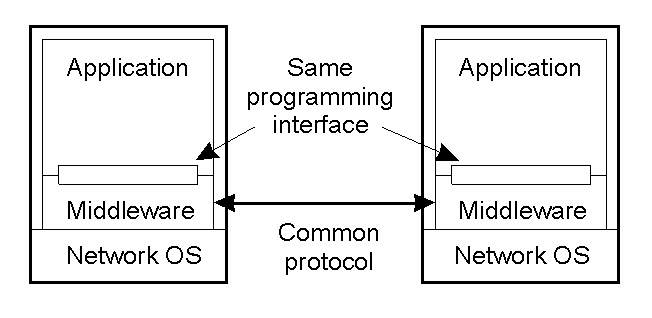
\includegraphics[width=1\textwidth]{pics/middlewareComm.jpg}
	\caption{Middleware based system [Tanenbaum1]}             
	\label{fig:MddlewareComm}
\end{figure}  
%**********************
%**********************
\begin{figure}[!hbt]                               
	\centering                                           
	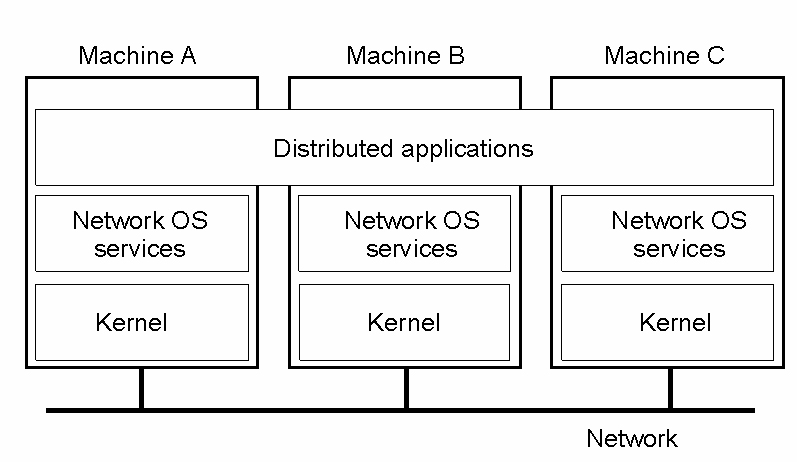
\includegraphics[width=1\textwidth]{pics/middlewareGeneral.jpg}
	\caption{Middleware based system [Tanenbaum1]}             
	\label{fig:MiddlewareGeneral}
\end{figure}  
%**********************
If you take a look from the top, from the users point of view he will get a homogenouse view of the system. Using the applications and developing them you won't have to take care about the underlying hetrogenity. It provides a single and coherent view to it's users. The rise of client/server application architectures where system components access remote infrastructure and functionality to accomplish their own tasks has led to the need to decouple communication parties to assure the need for scalability in the current IT infrastructures.
\\\\
To get a better understanding take the example from [Tanenbaum1]:
\\\\
Orders are placed from different types of clients like notebooks connected to the network, from the telephone network or cell phones. Those incoming orders are processed by a workflow system and the result is a new internal shipping order from the planning department and a billing order from the accounting. The users are not aware at all where those forwarded orders physically come from it appears that they are from a single central authority.
%**************************************************************************************
\subsection{Middleware Layer}
%**************************************************************************************
What makes this possible is the additional middleware layer that helps to hide the hetrogenity of the underlying platforms and improves transparency. The DOS is not intended to handle a collection of independent computers and a NOS doesn't provide a  view of a single coherent system. There are several models/paradigms describing the middleware layer:
\begin{itemize}
	\item Plan 9 was the first approach which treats everything as a file because that can be shared by several processes in the unix world and the communication is reduced to accessing files.
	\item Remote Procedure Calls (RPCs) allows to call functions and pass parameters on a remote machine. The callee doesn't know anything about the location of the remote function which can be on a machine physically somewhere else on the world.
	\item Distributed objects describes the method to invoke objects in a transparent way on remote machines by providing interfaceses of those objects.
	\item The message oriented paradigm takes care about providing the same communication facilities so that systems can talk to each other. The content of the information itself is ignored by these type of middleware models.
\end{itemize}
%**************************************************************************************
\subsection{Communication Paradigms}
%**************************************************************************************
There are different communication paradigms we have to be aware of before continuing:
\begin{itemize}
	\item \textbf{Transient communication} stores a message only as long as the sender and receiver is up and running.  
	\item \textbf{Persistent communication} on the other hand stores a message as long as the receiver retrieves it.
	\item \textbf{Asyncronouse communications} characteristic is that it sends a message and doesn't wait for a notification so it can keep on working without a halt.
	\item Applying \textbf{Syncronouse communication} will result in a delay for the sender until a received notification will come in from the receiver. 
	\item \textbf{Broadcast} means that a sender is communicating to multiple receivers.
	\item \textbf{Point to Point} communication is simply that one communication links has been established between sender and receiver.
\end{itemize}

Today the message oriented middleware paradigm has become one of the communication pillars of todays enterprise systems. It is the most common communication facility for exchanging information. There are different ways of organizing message oriented middlewares, but the most important is the message queing type. 
\\\\
\textit{Message-queing systems provide extensive support for persistent asynchronous commuication} [Tanenbaum1]
\\\\
In practice each application has got it's own message queue or several applications share one queue. This enables applications to communicate with eachother by inserting messages into specific queues using message-queing systems. This allows a loosely-coupled communication between systems. The inserted messages are pending in the queue as long as the receiver fetches it from the queue. So neither the sender or the receiver client has to be online if a message has been deployed in a queue. An important fact is that usually message-queueing systems don't gurantee the delivery of the sent messages. However there are mechanisms available in a variety of products to ensure the success of message transactions. This message based style communication bears the potential to integrate new autonomous, heterogeneous components into complex systems that are easy to evolve and scale \cite{LudgerFiege05}.
\\\\
As messages can contain any form of data the integration into a distributed system can lead to problems as applications provide different data formats. Message Brokers are an important application to act as a gateway between message-queuing systems. It transforms messages into a format that can be read by the different communication partners.
\\\\
The layering according to [Tannenbaum1] is a very simple point of view as he only wants to show how a middleware can enable a transparent and single coherent view of a system. David Luckham introduces a slightly deeper granularity of the high level overview of an distributed, event-driven system in order to be able to understand the importance of events for an enterprise.
\\\\
\textit{Layered IT systems present another dimension in the search for new ways to understand the events that happen in them.} [Luckham05]
\\\\
%**********************
\begin{figure} [h]                        
	\centering                                           
	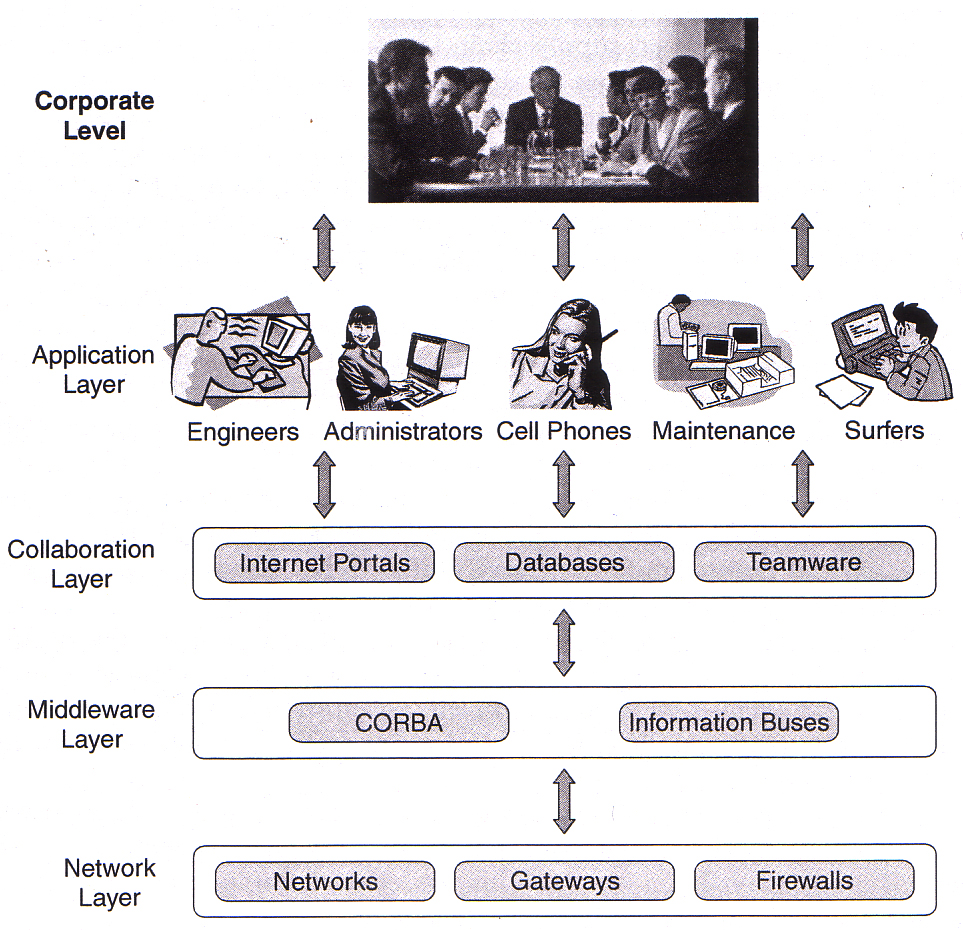
\includegraphics[width=1\textwidth]{pics/corporateLayer.jpg}
	\caption{Enterprise System Layering [Luckham05]}             
	\label{fig:EnterpriseSystemLayer}
\end{figure}  
%**********************
\begin{itemize}
	\item \textbf{Corporate Level:} At this layer enterprises plan and transact their business. Applications like accounting, inventory, spreadsheets, e-mail clients, calendars, webbrowsers and in general interfaces to other services belong in here.
	\item \textbf{Application Layer:} At this layer events are generated on a high level by the user where they signify activities like sending an e-mail. Actually many events generated at this layer are not simply one event rather they are aggregated to a high level event from the events generated by the layers underneath.
	\item \textbf{Collaboration Layer:}: This layer provides the the basic infrastructure for applications like databases, e-mail servers, web servers and so on. The line between the application layer and the collaboration layer can be blury.
	\item \textbf{Middleware Layer:} As mentioned above this is a very important part because it lets enterprise systems talk to each other.
	\item \textbf{Network Layer:} This layer is the basic layer where everything builds on top of it. At this layer only low level events are generated to transport information from A to B.
\end{itemize}

%**************************************************************************************
\subsection{On events}
%**************************************************************************************
As we talk quite a lot about passing messages back and forth in enterprise systems what meaning has an \textit{event} exactly? 
\\\\
In context of computer science an event is used to control the flow of a program. A well known application are user interfaces where triggered user interface elements generate events to start a processes.
\\\\
According to [Luckham05] an event is defined as:
\\\\
\textit{An event is an object that is a record of an activity in a system. The event signifies the activity. An event may be related to other events.}
\\\\
Ludger Fiege describes an event in his thesis as:
\\\\
\textit{Any happening of interest that can be observed from within a computer is considered an event}\cite{LudgerFiege05}
\\\\
For better understanding we follow \cite{Lamport78} and assume that we have a distributed system holding processes for receiving and sending messages. The dot represents occured events and the dotted line represents a message. The vertical direction represents the time and the horizontal the space dimension.
%**********************
\begin{figure}                         
	\centering                                           
	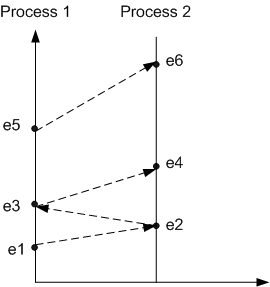
\includegraphics[width=0.6\textwidth]{pics/lamportEvent.jpg}
	\caption{Events and Messages}             
	\label{fig:LamportEvent}
\end{figure}  
%**********************
There are three aspects an event covers [Luckham05]:
\begin{itemize}
	\item \textit{\textbf{Form:} An event is an object containing attributes or data components.}
	\item \textit{\textbf{Significance:} An event signifies an activity}
	\item \textit{\textbf{Relativity:} An activity is related to other activities by time, causality and aggregation.}
\end{itemize}
Furthermore an event ussually contains an unqiue id and a timestamp to mark the creation of that event. 
\\\\
An example for events used in our system as a simulation model would be an OrderReceived event that signifies the activity of a posted order for some products:
\\\\
%{\MyCode 
\begin{lstlisting}[caption=OrderReceivedEvent]{OrderReceivedEvent}
<OrderReceived>
	<OrderId>14765</OrderId>
	<DateTime>2005-10-31T11:31:02</DateTime>
	<DeliveryDate>2005-11-12T06:00:00</DeliveryDate>
	<Destination>Madrid</Destination>
	<ProductCollection>
		<Product>		
			<ProductId>Arzeutic</ProductId>
			<Amount>700</Amount>
		</Product>	
	</ProductCollection>
</OrderReceived>
\end{lstlisting}
%} 
Events are generated from different sources and different types. Normally they use some standard like the XML format. The received events must be transformed into higher level form in order to be able to work with them. This transformation is provided by adapter compontents.
%**************************************************************************************
\subsubsection{Relationsships}
%**************************************************************************************
According to [Luckham05] there are three important relationships between events:
\begin{itemize}
	\item \textbf{Time:} Relates events according to their temporal occurence
	\item \textbf{Cause:} Relates events according to their causal relationships. A causal relationship is given when an event a caused another event b in a direct or indirect way.
	\item \textbf{Aggregation:} Aggregates event to high level events based upon different criterias like time, causality or content patterns.
\end{itemize}
Following Luckhams [Luckham05] proposal that a timestamp defines the time relationship between events is not as easy as he says that you can determine by the time dimension that \textit{event A happened before event B}. Leslie Lamport adresses this problem \cite{Lamport78}:
\\\\
\textit{In a distributed system, it is sometimes impossible to say that one of two events occured first. The relationship "happened before" is therefore only a partial ordering of the events in the system.} \cite{Lamport78}
\\\\
The happens-before relation "$\rightarrow$" can be defined for following situations:
\begin{itemize}
	\item If a and b are events in the same process, and a comes before b, then a $\rightarrow$ b.
	\item If a is an event sending a message from one process and b is an event receiving the message from another process then a $\rightarrow$ b.
	\item The happens-before relation "$\rightarrow$" is transitive: a $\rightarrow$ b and b $\rightarrow$ c then a $\rightarrow$ c. 
	\item If two events, a and b, are distinct they are called concurrent which means that you can't say which event happend first. In ohter words it means that if the events a and b happen in different processess and they do not exchange messages then a $\not\rightarrow$ b and b $\not\rightarrow$ a.
\end{itemize}
%**********************
\begin{figure} [!h]                
	\centering                                           
	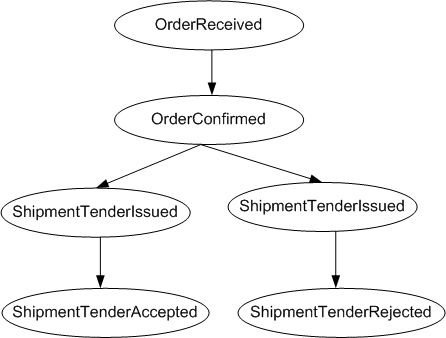
\includegraphics[width=0.7\textwidth]{pics/acyclicEventGraph.jpg}
	\caption{Directed acyclic graph of an event history}             
	\label{fig:dag}
\end{figure}  
%**********************
Martin Flower is addressing another important issuse regarding timing [http://martinfowler.com/eaaDev/TimePoint.html]. Date and Time information can come in different  precision formats. You could get a date on a daily precision and you could get it on msec precision level depending on your application. But as you work with events collected from different sources this could become a problem especially in distributed environments over the Internet where different time zones come in too. Furthermore the question arises which event occurence do you count? The one where the event happened physically on a machine or when it has been processed somewhere else? This kind of questions have to be considered when building a system to process or collect events from different distributed sources.
\\\\ 
In general a \textbf{causal relationship} determines that an event A caused another event B. As we have seen in our layered enterprise according to [Luckham05] events flow through these layered environment triggered by the user or another system at the top level and consequently transformed into lower level events down to the bottom causing other events to fire. This event flow is called \textit{vertical causality} and tracks down how high level events beginning from the business level manifest in lower layers. This is important to understand how these events are decomposed the way down in ordered to be able to create meaningfull aggreagations out of the masses of low level events. On the other hand Luckham talks about \textit{horizontal causality} that tracks the causal relationships between events at the same level. Causal relationships are transitive and asymmetric and can be represented as directed acyclic graphs. 
\\\\
\textit{Recognizing or detecting a siginificant group of lower-level events from among all the enterprise event traffic, and creating a single event that summarizes in its data their significance, is called event \textbf{aggregation}.} [Luckham05]
\\\\
Aggregating events is a difficult tasks as it needs a technology that can recognize patterns of events through different layers. But if such an aggregation facility is set up and running it can be a powerful source of tracking down causalities between events.

%**************************************************************************************
\subsection{Eventbased systems}
%**************************************************************************************
The term of event-based systems is used in many fields in an ambigious and varying way. As we have decribed several messaging architectures like the persistent, transient and asychronouse way to deliver messages to a client there is a distinct line between simple message exchange and event-based systems. The exhaustive trend of using distributed system architecture to support highly automated data processing has led to the concept of client-server architectures that brough major drawbacks with it. A classic client-server architecture, where system compontents access remote functionality to acomplish their own tasks, is often a synchronouse communication between the server and the client. That leads to tight coupling and affects the scalability of such architectures. Several middleware extensions addressed this problem by allowing to use asynchronous messaging in an either persistent or transient way using the mentioned message queing techniques. 
\\\\
In an event-based environment we have components communicating with eachother by sending and receiving event notifications. There are mainly two interacting components the \textit{consumer} and the \textit{producer}. The consumer is subscribing to certain notifications and the other component, the producer, is publishing notifications about various topics. A notifications service dispatches the notifications from the producer to the subscribed consumer. This notification service makes it possible to create easily loosly coupled and scaleable infrastructures as none of the components have to know about eachother. The notifications itself is created by observing special occurrences that are a point of interest. The subscription of consumers is a list of certain notifications the consumers wants to receive by the notification services. The subscription mechanism could be just a filter function or a more sophisticated notification selection mechanism including metadata descriptions. A channel would represent such a bundle of notifications that a consumer could subscribe and a producer could select to distribute its notifications.
\\\\
%**********************
\begin{figure} [ht]                
	\centering                                           
	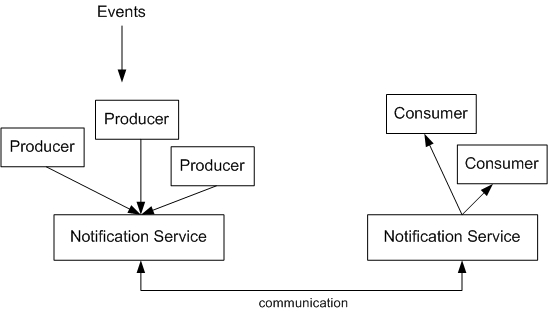
\includegraphics[width=1\textwidth]{pics/eventBasedConsumerProducer.jpg}
	\caption{Event-based notifications}             
	\label{fig:event-basedNotifications}
\end{figure}  
%**********************
\\\\
As you can see there is the major drawback of missing filtering, aggregation and colleration services like mentioned in the introduction. Actually there is no big deal to set up a message queue for a component or a system to receive specific event notifications from a channel. Let assume that you have a component or a system subscribed to a shipment tracking channel that sends continouse notifications about the current status of a package and another subscription to a channel that notifies about shipment audits. The system would be able to handle those received events according to its assigned tasks in ways like: 
\begin{itemize}
	\item \textit{The shipment xy has been audited and a damaged product has been indentified.} The system can book product xy from shipment xy as damaged.
	\item \textit{The shipment xy has been delivered.} The system can book the shipment xy as finished.
	\item \textit{The shipment xy is currently on road between Vienna and Linz.} The system can react in sense that it updates a some location tracking systems used.
\end{itemize}

There is a wide range of options how to deploy systems even in ways that systems can react in very intelligent ways, but in sense of gathering high level business information or tracking business processes it won't be possible as you would need a facility that collects all events and it would even need access to historic data in some cases to find out for example what caused to failed the shipment from the example above. If you would want to create high level overviews of that shipment you would need correlation information about those events that belong to one shipment or you would need aggregation functionality to create more abstract groupings of those information. Another problem dimension is that todays business environment requires a fast paced  decision infrastructure based on up-to-date information. For long people complied with that decision making does not require actual data instead it needs huge amounts of historical information collected in data warehouses. 
\\\\
\textit{[...] strategic decision makers are being exposed to the huge inflows of data and information from their resources and they are under rigid time constraints to make the right decisions.} [NguyenSchieferTjoa05]
\\\\
According to Hackathrone the business value of taking an action goes down after an event happend (see Figure \ref{fig:event-basedNotifications [Hackathorn02]}).

%**********************
\begin{figure} [ht]                
	\centering                                           
	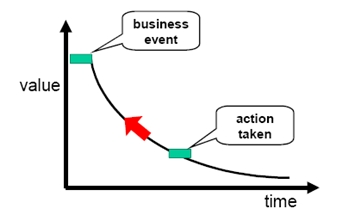
\includegraphics[width=0.8\textwidth]{pics/businessValue.jpg}
	\caption{Event business value}             
	\label{fig:event-basedNotifications [Hackathorn02]}
\end{figure}  
%**********************
%**************************************************************************************
\subsection{Related work to event-based systems}
%**************************************************************************************
Currently there is quite a lot of work going on in the design and application of event-based system support and correlatin systems. This chapter will introduce some of the most prevalent systems.

%**************************************************************************************
\subsubsection{Senactive InTime - Sense and Response Architecture}
%**************************************************************************************
%**********************
\begin{figure} [ht]                
	\centering                                           
	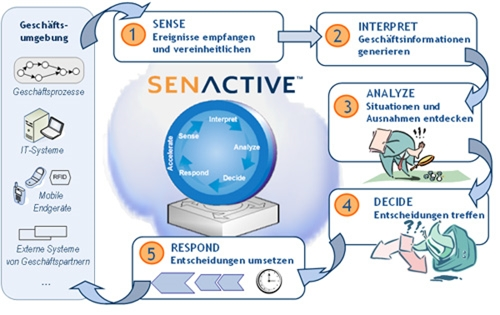
\includegraphics[width=1\textwidth]{pics/senseAndResponseSenactive.jpg}
	\caption{InTime Sense and Response Architecture \cite{SenactiveWebpage}}             
	\label{fig:senseAndResponseSenactive}
\end{figure}  
%**********************
The basic idea behind the \textit{Sense and Response Service Architecture} used in Senactive's InTime product is to monitor IT- and businessprocesses in sense and response loops. This architecture allows to gather business intelligence data and make decisions based on actual information. Real-time event sources are connected to the system by event adapters and fed into \textit{Sense and Response loops} which is divied into 5 phases. 
\\\\
The 5 phases in detail (see Figure \ref{fig:senseAndResponseSenactive}) \cite{NguyenSchieferTjoa05} :

\begin{itemize}
	\item \textbf{Sense}: Continouse capturing of of events and unification by the sense and response architecture.
	\item \textbf{Interpret}: The events will be transformed into business information like performance indicators, business situations and exceptions.
	\item \textbf{Analyse}: Analysis of interpreted business information to preditct performance and risks if the business environment changes.
	\item \textbf{Decide}: Proposal for the best business situation and the accroding actions to be done either automated or by involving humans.
	\item \textbf{Respond}: Communicating the decision made in the last step to change the business environmant.
\end{itemize}

The processing, transformation and the relationshipdefinition steps can be defined for every organisation using an event processing model for modeling these sense and response loops.
\\\\
The system is capable of detecting exceptional business situations and can react on them by generating warnings or take measures by itself to prevent damages like fraud. The InTime product is also capable of correlating events and aggregating events from it's various sources. This product would help customers to monitor their event-driven enterprise systems from a high level perspective to gather financial ratios, to trace down occured problems or to use it for decision making based on real time information. As this product can react proactivly on given business situations in its \textit{decide cycle} it can change business situations autonomously based on rules and provided information. The change of business situations can be performed in an event-based manner again. 
\\\\
This \textit{Sense and Response Service Architecture} can be used to satisfy real-time business intelligence architecture requirements as it can be used as a real-time data cache that serves as a staging area for datawarehouse updates and analytical services. More on zero-latency data warehousing and real-time business intelligences has been addressed here \cite{TjoaNguyenKickinger04}, \cite{NguyenSchieferTjoa05} and \cite{ThoManhNguyen05}.
\\\\
A useful feature of Senactives InTime is an event simulator that can generate events to create simulations to test event workflows or to generate event-based data for other purposes. This feature has been used for this diploma thesis to simulate logistics service prodiver based upon some special exceptional stories created. 

%**************************************************************************************
\subsubsection{RAPIDE}
%**************************************************************************************
RAPIDE is an event pattern language developed at Stanford University by the Program Analysis and Verification Group under the lead of David Luckham. RAPIDE is a declerative computer language that enables the specification of patterns of events. The syntax of of RAPIDE is basically like todays languages like Java or C\#. RAPIDE allows the specification of patterns that form relationships between events by causal, content or temporal constraints. This language has the feature to add pattern rules during runtime while events are collected according to the given pattern rules and processed by given action statements. Rapide is capable of aggregating high level events out of a collection of correlated events.
\\\\
It has a rich set of features \cite{Luckham05} like:

\begin{itemize}
	\item Definition of Event types.
	\item Event pattern definition
	\item Pattern operators for modeling relationships between events.
	\item Temoral operators to specify the timeing of events.
	\item Pattern macros for building more complex patterns.
\end{itemize}

According to \cite{LuckhamManensPark} RAPIDE is a good approach to test and simulate business process as it is easily possible to track causal relationships and to detect contraint violations during simulation. 

%**************************************************************************************
\subsubsection{Generalized Event Monitor - GEM}
%**************************************************************************************
%**********************
\begin{figure} [ht]                
	\centering                                           
	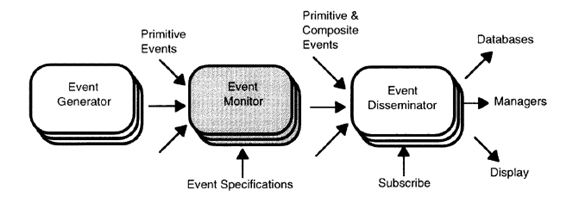
\includegraphics[width=1\textwidth]{pics/GEM.jpg}
	\caption{Event monitoring components \cite{GEM95}}             
	\label{fig:gemEventMonitoringComponents}
\end{figure}  
%**********************
The Generalized Event Monitor (GEM) is an interpreted declarative rule-based event monitoring language which allows to specify high-level events out of different nodes in a distributed system. The purpose of GEM is to monitor operations of distributed systems to support managment decisions and control network behaviour. The monitor is capable of applying filters and to correlate events according to predefined rules. GEM's pecification contains the type of the vents to be collected, a pattern that has to be matched and an action to be performed. GEM's specification is very powerful as it allows the definition of triples (format, composite event definition and actions to be defined). Moreover it is possible to modify the GEM monitors state. The main drawback is that it does not support to model causal relationships between events which result in a lack of defining patterns based on causalities between events. For further details see \cite{GEM95}.
%**************************************************************************************
\subsubsection{HP-ECS Event correlation service}
%**************************************************************************************
%**********************
\begin{figure} [ht]                
	\centering                                           
	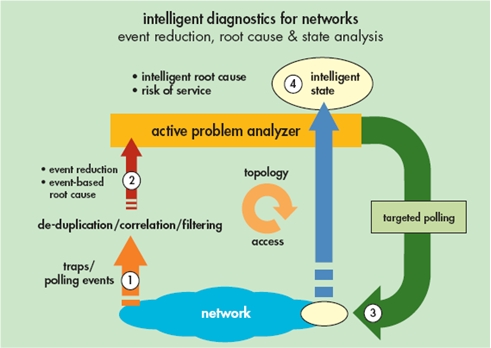
\includegraphics[width=1\textwidth]{pics/openView.jpg}
	\caption{HP-ECS OpenView \cite{OpenViewHP}}             
	\label{fig:openViewHPECS}
\end{figure}  
%**********************
Hewlett Packard provides a commerical event correlation product for correlating events coming from various system levels like the lower network layers, enterprise systems and application or database systems. HP-ECS correlates events by defineing correlation circuits either with a sophisticated GUI. These correlation circuits are a set of nodes connected to each other where the events pass through.  
\\\\
Events can be passed through intermediate nodes in a circuite that provides different features like:
\begin{itemize}
	\item temporal filters
	\item causal filters
	\item content filters
	\item in general event monitoring
	\item sequential event contructs 
\end{itemize}

HP-ECS has a major flaw because it is not usable for generic event correlation as it only supports correlation for SNMP and CMIP events.

%**************************************************************************************
\section{Scope of this diploma thesis}
%**************************************************************************************

We have seen in the previous chapters which impact events have got in todays decision making processes and what value it creates for process managment especially in large and global oriented enterprises. E-Business and E-Markets have created a global playground for automated workflow systems which results in a huge traffic flow of information between corporate networks and department systems. The lack of monitoring these events in a sense of correlating them, creating causal relationships or aggregate them to high level events is still a problem that is currently challenged by academic and commerical oriented institutions. Some of them like Senactive's Sense and Response Architecture provides the ability to monitor event flows and proactivly react on them to change the business processes based on real-time information provided by the various enterprise systems. This is a major step towards real-time enabled enterprises that can challenge the requirements of todays highly dynamic business world. 
\\\\
The core of this diploma thesis does not go in first place into event-based processing problems like creating sophisticated causal trackings or correlation algorithms. This thesis is about a system that enables the historic view of collected historic event streams that have been preprocessed by Senactives InTime Sense and Response Architecture. As Intime can react proactivly on given business situations based on event constellations and defined rules it can rearrange business processes to stear the business environment and processes into a given direction. This will result in a chain of newly triggered event flows which join back to the control loop. InTime is capable or correlating events according to predefined rules and delivers causal tracking of events. 
\\\\
The system developed in this diploma thesis is collecting those \textit{catched} events and creates a full text index over them to enable a Google like search experience for investigation purposes. The major application of this system is to offer the user a toolset to discover different aspects of business processes based on event correlations. This system has evolved over several stages to clarify which architecture would be the best solution to provide this kind of search and discovery experience to a user and at the same time to lay the foundation for further work in the area of event mining and correlation discovery. 
%**************************************************************************************
\newpage
\section{Searching for correlated business information}
%**************************************************************************************

%**************************************************************************************
\subsection{Information Findability}
%**************************************************************************************
According to \cite{Morville05} findability is described by following aspects:

\begin{itemize}
	\item \textit{The quality of being locatable or navigable.}
	\item \textit{The degree to which a particular object is easy to discover or locate.}
	\item \textit{The degree to which a system or environment supports navigation and retrieval.}
\end{itemize}

Google has shown the world that searching the web does not have to be based on simple keyword matchings or word frequency countings. It introduced a completle new way of rating weppage contents and to calculate the best hits out of some search terms provided by the user. Google's commercial success has proven the world that this way of finding information is the right one at least for the moment as long as noone else comes with a better idea. 
\\\\
The look and feel of Google like finding and retrieving information has become a defacto standard and numerous applications integrate full text indexing algorithms and methods into their applications to provide a search based access to information and data. These applications don't necessarliy concentrate on finding webpages it's applied on a variety of information like office documents, products, flight schedeules or even free available source code. People tend to go away from the classic topologic of classifying information into tree like catalogous and let the user to navigate through these structures to get their desired information. A good indexing and retrieval mechanism allows the users to find and access information by typing some terms into a textbox and a ranking algorithm calculates the best hits out of the found information to present the most relevant information. This way of organising the access to information has become a great success as numerous applications has proven like koders.com, Google Desktop Search and Apple's Spotlight for instance. 
\\\\
\textit{Of course, access doesn't simply require us to make decisions in more areas of our lives. It also changes the game by inviting us to make informed decisions more often.} \cite{Morville05}

%**************************************************************************************
\newpage
\subsection{Background}
%**************************************************************************************

% welchen bedeutung hat event cloud? siehe scope
% was kann der Benutzer damit machen?
% Grundlage f�r Eventmining und correlation finding
% Geeignete Architektur f�r so eine Anwendung finden
% Fokus auf freie Technologien

Event Cloud is the name of the developed application whose main purpose is to provide a search interface to its users to allow them to search for simple and correlated events in an efficient way.  The representation of the search results is a major feature that allows its user get the most relevant hits according to the given search criterias. Furthermore it provides functions to exclude unwanted event and correlation types from the found result set and it allows to create filters over events and their correlations. As not every person is interested in all types of occured events and correlationsets it is possible to create and edit roles for different user profiles that will reduce the information pool to a desired managable pool of events and correlations. Event Cloud provides the user the option to to dig down to event levels or to go up to correlation levels according to the selection from a found resultset. 
\\\\
Basically Event Cloud has implemented two Search types that allows a user to query for either events or to search through whole event correlations. Using the latest Java high-performance text search engine library Lucene and the powerful open source database Postgres allows to index and search the event repository in a fast and efficient way. The system is supported by the Spring framework to bind the components together.
\\\\
Basically Event Cloud consists of three main functions: 

\begin{itemize}
	\item Extracting and transforming event data from the source system and integrate them into Event Cloud's own data structure.
	\item Full text index over simple and correlated events.
	\item Search functionality including a sophisticated query syntax and various filter functions
\end{itemize}

This functionalitie should provide a powerful toolset to facilitate the discovery of different aspects of business processes based on event correlations provided by a Google like experience. 
\\\\
This diploma thesis was supported by Josef Schiefer and Senactive by providing Intime for the basic infrastructure and support throughout the whole developing process. Especially the simulation of business processes to gather test data in form of generated events was done by the Intime product.

%**************************************************************************************
\newpage
\subsection{Search Concepts}
%**************************************************************************************
% Das Suchen ist der zentrale Teil daher muss man bestimmte Suchkonzepte unterscheiden die
% vom System unterst�tzt werden.
The subsequent chapters will give an conceptual overview of the search type features provided by Event Cloud.

%**************************************************************************************
\subsubsection{Rank 1}
%**************************************************************************************
The Rank 1 search is simple full text search over all searchable attributes of an event. The user is able to put down a search query consisting of several search terms and boolean operators according to Lucenes BNF query syntax. The result will be a list of events that matched the given query. 
\\\\
The Rank 1 search is pretty straight forward like you would search documents on the internet using any search engine available. 
\\\\
Take a look at the example (Figure \ref{fig:rank1searchExample}) where we have several events in our repository. The user queries for the terms "Paris London Szabolcs" and gets back the events TransportEnd and TransportStart as these terms occured in those events ordered by the most relevant hits. No boolean operators have been applied in this query example. If the user would have entered a query like "szabolcs AND Paris" he would have received events where the terms Paris and Szabolcs would have occured. For more details take a look at the query syntax as this is not in the scope of this chapter.
%***********************
\begin{figure}[ht]                                  
	\centering                                           
	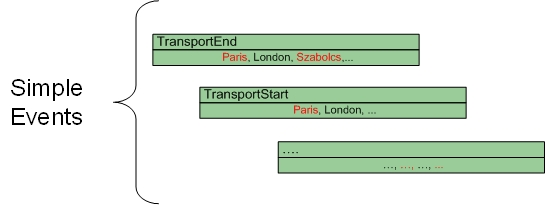
\includegraphics[width=1.0\textwidth]{pics/rankOneSearchExample.jpg}
	\caption{Rank 1 search example}             
	\label{fig:rank1searchExample}
\end{figure}            
%***********************      
%**************************************************************************************
\subsubsection{Rank 2}
%**************************************************************************************
At the current point the heart of Event Cloud is the Rank 2 search which is an extension of the Rank 1 search. The difference between Rank 1 and Rank 2 search is that this search type is not looking at events at an atomic level rather it searches over whole correlations of events (Figure \ref{fig:rank2correlation}). By executing a Rank 2 search the query will go over whole correlationsets of events instead of looking only at events like in the Rank 1 search type. 
\\\\
%***********************
\begin{figure}[h]                                  
	\centering                                           
	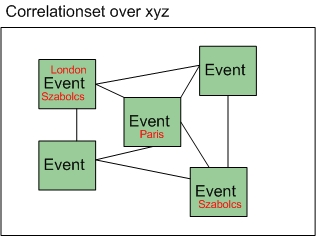
\includegraphics[width=0.7\textwidth]{pics/rankTwoSearchExample.jpg}
	\caption{Rank 2 search example}             
	\label{fig:rank2searchExample}
\end{figure}            
%***********************   
If a user puts down a search query consisting of terms like "Paris London Szabolcs" the search engine will retrieve correlations consisting of events that matched these terms (Figure \ref{fig:rank1searchExample}). That means that you will get back a correlation whose event attributes contain either Paris, London or Szabolcs. Correlationsets whose Events would not contain the terms "Paris London Szabolcs" would not be considered. If for instance a correlationset is consisting of eigth events and only one event contains the search terms it would be still a hit but maybe a bad one depending on the other found hits.
%***********************
\begin{figure}[h]                                  
	\centering                                           
	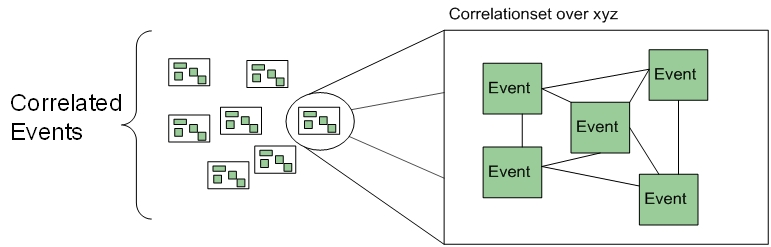
\includegraphics[width=1.0\textwidth]{pics/rankTwoCorrelation.jpg}
	\caption{Event correlation}             
	\label{fig:rank2correlation}
\end{figure}            
%*********************** 
   
%**************************************************************************************
\subsubsection{Rank 3}
%**************************************************************************************
This type of search is not implemented in the current work as it is a very complex topic and beyond the scope of this diploma thesis. For the sake of completness I want to give a brief overview about this event search type. The Rank 3 is searching over correlations like the Rank 2 search but instead of using direct correlations between events it searches over indirect correlations between correlationsets. It is actually the same like the Rank 2 but one aggregation level higher and the result hits are additionally evaluated by a distance factor of these indirect correlations.
\\\\
The challenge behind this type of correlation search is to discover indirect correlations between events and to implement an effective search alorithm to rank the most relevant hits. This technique could become a performance eating task as you have to find a way to consider a higher aggregation level when querying for events.
%***********************
\begin{figure}[h]                                  
	\centering                                           
	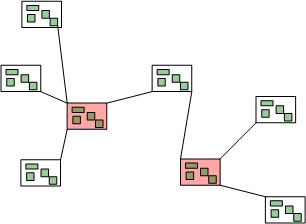
\includegraphics[width=0.5\textwidth]{pics/rankThreeSearchExample.jpg}
	\caption{Rank 3 search}             
	\label{fig:rank3searchExample}
\end{figure}            
%***********************  
%**************************************************************************************
\newpage
\subsection{Architecture}
%**************************************************************************************
% Hier fangen jetzt die Details an! High level Architektur + Technologien genau beschreiben
% High Level overview mit Bild und kurz die Komponenten beschreiben und wie sie zusammenspielen
% simulator f�r eventsimulation kurz erw�hnen und details dann beim Simulator abschnitt selber schreiben.
%**************************************************************************************
\begin{landscape}
\subsubsection{High level overview}
%**************************************************************************************
%***********************
\begin{figure}[ht]                                  
	\centering                                           
	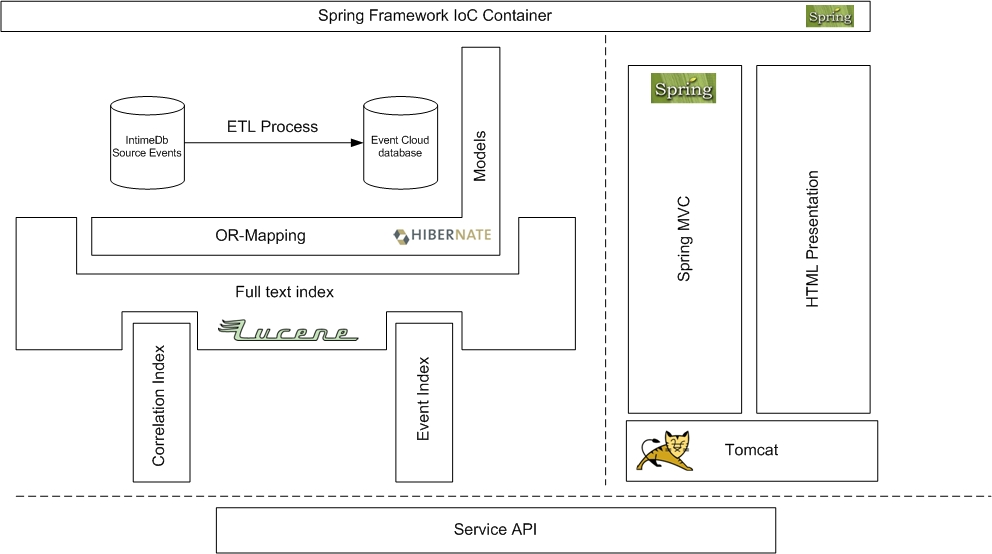
\includegraphics[width=1.2\textwidth]{pics/EventCloudHighLevelOverview.jpg}
	\caption{Event Cloud High Level Overview}             
	\label{fig:eventCloudHighLevel}
\end{figure}            
%***********************                       
\end{landscape}
%**************************************************************************************
\subsection{Searching}
%**************************************************************************************
%**************************************************************************************
\subsubsection{Query Syntax}
%**************************************************************************************
Event Cloud is using Lucene's sophisticated query parser to provide a full featured query syntax to allow the creation of complex queries for searching and retrieving events and their correlations. 
\\\\
The formal query grammar definition \cite{LuceneQueryParserAPI}:
\begin{lstlisting}
Query  ::= ( Clause )*
Clause ::= ["+", "-"] [<TERM> ":"] ( <TERM> | "(" Query ")" )
\end{lstlisting}
A clause can contain either a Term expression or another nested Query. There are two distinctions between terms. There can exist a \textit{single term} like "hello" or "test" or a term can be a \textit{phrase} like "hello world" enclosed by double quotes. It is possible to combine multiple terms with boolean operators \cite{LuceneQueryDescriptionPage}. The predefined Boolean connector configured in Event Cloud for Terms is the OR operator.
\\\\
Some basic query examples are described in the table \ref{fig:rank1LuceneQueryExamples} for getting started.
\\\\
However the QueryParser is capable of much richer functionality like Fuzzy Searches and and Proximity Searches. They don't have a big importance in querying but it can be powerful tool. For example it is possible to create a fuzzy search based on the Levenshtein distance using the tilde ~ symbol plus a proximity number. For example you can search for "\textit{java~}" and it will return documents that are similar to java like lava. You can adjust the proximity by adding a value next to the tilde symbol like java~0.8. The default proximity number is 0.5.
\\\\
Another noticeable minor future is the possibility to define the relevance of search terms in a query with the carot operator $\wedge$ and a number that specifies the importance of the word. For instance if you search for "\textit{Paris$\wedge$4 London}" it will make Paris more relevant than London. The default relevance value is 1.
\\\\
Further details on this topic can be found here \cite{LuceneQueryDescriptionPage} and here \cite{LuceneQueryParserAPI}

\begin{table}[!hp]
	\begin{tabular}{|p{4cm}|p{8cm}|}
		\hline \textbf{Example} & \textbf{Description} \\
		\hline \textit{Paris} & Query will return events containing "Paris" in an Attribute. \\
		\hline  \textit{Paris London} & Query will return events containing either "Paris" or "London" in an Attribute. \\
		\hline  \textit{Paris OR London} & Query will return events containing either "Paris" or "London" in an Attribute. \\
		\hline  \textit{Paris AND London} & Query will return events containing "Paris" and "London" in an Attribute.\\
		\hline  \textit{(Paris OR London) AND Szabolcs} & Query will return events containing "Paris" or "London" but they must contain "Szabolcs".\\
		\hline  \textit{+Paris +London} & Query will return events containing "Paris" and "London" in an Attribute.\\
		\hline  \textit{+Paris -London} & Query will return events that must contain "Paris" and it is not allowed that this event contains "London" in an Attribute.\\
		\hline  \textit{+Paris NOT London} & Query will return events that must contain "Paris" and it is not allowed that this event contains "London" in an Attribute.\\
		\hline  \textit{Par*} & Query will return events containing words that start with "Par" - for instance Paris.\\
		\hline 
	\end{tabular}
	\caption{Query Examples}
	\label{tab:LuceneQueryExamples}
\end{table} 

% Verwendete Patterns beschreiben
%	Facade Pattern
% 	Inversion of Control
%	Code injection

% verwendete Technologien beschreiben:
% Tomcat
% Hibernate als OR Mapping
% Datenbank Postgres
% Spring
% MVC Konzept
% Spring MVC
% Lucene



% ETL Prozess
% 	Hibernate als OR Mapping
%		Wie schauen definition files aus
%	Datenbank Postgres

% Indexing 
%	Lucene index structur
%	Verwendung von Lucene als Codebeispiel
%	Caching Themen
%	Darauf eingehen wie man

% Suche
% 	web interface 
%	Spring framework
%	Spring MVC - MVC Konzept im allgemeinen

% Beschreibung der API
%	UML Bilder und beschreiben was was macht

%**************************************************************************************
%\newpage
%\subsubsection{Evolution}
%**************************************************************************************

%**************************************************************************************
%\newpage
%\subsection{Performance}
%**************************************************************************************

%**************************************************************************************
%\newpage
%\subsection{Simulation}
%**************************************************************************************

\newpage
\bibliographystyle{alpha}
\bibliography{eventcloud}

\end{document}
